\documentclass[12pt]{article}
\usepackage[english]{babel}
\usepackage[utf8x]{inputenc}
\usepackage{amsmath}
\usepackage{graphicx}
\usepackage[a4paper]{geometry}

\begin{document}
\begin{titlepage}

% definition of custom command for horizontal lines
\newcommand{\HRule}{\rule{\linewidth}{0.5mm}}

\center
% HEADING
\textsc{\LARGE University of Dublin,\\Trinity College}\\[1.0cm]

\includegraphics[width=0.2\textwidth]{logo.png}

\HRule \\[0.4cm]
\textsc{\Large ST2004 Optional Assignment}\\[0.25cm]
\textsc{\large Investigation into Probabilistic Processes of Monopoly}\\[0.1cm]
\HRule \\[0.4cm]
 
% AUTHORS
\begin{minipage}{0.5\textwidth}
\begin{flushleft} \large
\emph{Author:}
\\Edmond \textsc{O'Flynn} 12304742
\end{flushleft}
\end{minipage}
~
\begin{minipage}{0.4\textwidth}
\begin{flushleft} 
\large
\emph{Lecturer:} \\
Brett \textsc{Houlding} 
\end{flushleft}
\end{minipage}\\[3cm]

% DATE
{\large \today}\\[2cm] 

% LOGO
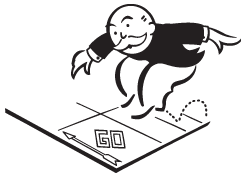
\includegraphics[width=0.4\textwidth]{monopoly_man.png}
\clearpage
\end{titlepage}

\newgeometry{top=1cm,left=1cm,bottom=2cm,right=1cm}
\tableofcontents
\addcontentsline{toc}{section}{References}
\thispagestyle{empty}
\cleardoublepage
\setcounter{page}{1}

\newgeometry{top=2cm,left=2cm,bottom=2cm,right=2cm}

\section{Introduction}
\subsection{What is Monopoly?}
Monopoly is a game where players traverse a board across 40 squares consisting of properties, which players may choose to purchase, as well as other spaces that offer chances and opportunities. Whilst the players move around the board with respect to independent dice rolls, the player may choose to buy and improve properties, or to pay rent to other players. The ultimate goal in the game is to cause the other players to become bankrupt, and to be the tycoon of the board.
\subsection{Rules}
Monopoly board traversal is the result of fundamentally rolling two independent dice and offsettings by the sum of the dice to the next end square.
\begin{enumerate}
  \item \textbf{Players start at Go} \hfill \\
  The player moves with respect to the sum of the dice faces clockwise around the board. If a player rolls a double, ie \{1,1\}, \{2,2\} ... \{6,6\}, the player may roll again.
  \item \textbf{Players Can Get Sent to Jail} \hfill \\
  On landing on a space, picking up a specific card, or rolling three doubles in a row, players may get sent to the jail tile.
  \item \textbf{Players May Buy Properties} \hfill \\
  On landing on a non-special tile, a player may choose to buy the land and receive rent if other players land on it. Players may also develop their properties if and only if they possess all colours within that tile group.
  \item \textbf{Winning Conditions} \hfill \\
  A player is deemed the winner if the other players become bankrupt, and only one player is left standing.
\end{enumerate}
\section{Model \& Simulation}
\subsection{Dice Rolls}
\begin{table}[h]
\centering
\label{my-label}
\begin{tabular}{cccccc}
(1,1) & (1,2) & (1,3) & (1,4) & (1,5) & (1,6) \\
(2,1) & (2,2) & (2,3) & (2,4) & (2,5) & (2,6) \\
(3,1) & (3,2) & (3,3) & (3,4) & (3,5) & (3,6) \\
(4,1) & (4,2) & (4,3) & (4,4) & (4,5) & (4,6) \\
(5,1) & (5,2) & (5,3) & (5,4) & (5,5) & (5,6) \\
(6,1) & (6,2) & (6,3) & (6,4) & (6,5) & (6,6)
\end{tabular}
\caption{Dice Roll Outcomes}
\end{table}
Given that a double has not been rolled on the first turn of the game, the following is the probabilistic outcome of landing on a square from starting position.

%normal graph here where #7 has the highest cumulative probability

Given that the outcome was not a double, there is a significantly higher chance of landing on a chance square, which is comparatively higher than landing on squares \#6 or \#8. Comparatively so, there is still a higher than 10\% chance of landing on squares 5-9.

In the case that a double has been rolled in which the probability of this is lower than rolling permutations of non-double dice. Doubles can be extremely powerful, thus changing the probabilistic outcomes of square landing probability. 

The Monopoly board itself is a 40x40 Matrix containing a mixture of tiles ranging from properties to varying cards that affect the player in different ways, both positively and negatively.

It is possible to traverse from starting position to \#35 in three rolls before succumbing to the \emph{No Speeding} rule, by which one must go to jail. Although small, in every 1000 rolls there will tend to be 4 triple double-rolls thrown.
\begin{align*}
\frac{1}{6}\approx16.7\% \quad &\textsl{of rolling 1 double}\\
\frac{1}{36}\approx2.8\% \quad &\textsl{of rolling 2 doubles}\\
\frac{1}{216}\approx0.4\% \quad &\textsl{of rolling 3 doubles and ergo get sent to jail} 
\end{align*}
Theoretically it is possible for double-rolls to tend to infinity, albeit exponentially this becomes probabilistically unlikely due to constant decreasing odds as well as the No Speeding rule.

The expected value of rolling 1 die is 3.5, therefore on rolling two dice, it's most likely that the expected value will be 7. It's also quite likely that your opponents will roll a 5, 6, 8 or 9 with respect to cumulative probabilities of dice rolling.
\subsection{Chance and Community Chests}
Monopoly contains 16 Community Chest cards, and 16 Chance cards. On landing on a community chest or chance card square, the player must abide by one of the five outcomes of varying probabilities on the cards.

\subsubsection{Chance Cards}
The 32 cards, 16 from Community Chest and 16 from Chance, drastically change the outcome of what happens within a game. By drawing a card from either deck, one of the following five results may happen:
\begin{enumerate}
  \item \textbf{Go to the Stated Tile} \hfill\\
  There is a $\frac{8}{16}$ chance of this.
  \item \textbf{Collect Money} \hfill\\
  There is a $\frac{3}{16}$ chance of this.
  \item \textbf{Pay Money} \hfill\\
  There is a $\frac{3}{16}$ chance of this.
  \item \textbf{Go to Jail} \hfill\\
  There is a $\frac{1}{16}$ chance of this.
  \item \textbf{Get out of Jail} \hfill\\
  There is a $\frac{1}{16}$ chance of this.
\end{enumerate}
Therefore, a probability of $\frac{9}{16}$ cards have the ability to transport the player across the board to another location, thereby altering the odds to being in another place to having a higher probability of landing. There is a total of three possible outcomes of spaces to land on within the weighting effect of certain spaces on the board:
\begin{enumerate}
  \item {Go to Jail}
  \item {Advance to Go}
  \item {Go Back Three Spaces} \hfill
  \item {Advance to Nearest Utility} \hfill
  \item {Advance to Nearest Railroad} \hfill
  \item {Advance to Boardwalk**} \hfill
  \item {Advance to Illinois Avenue**} \hfill
  \item {Advance to Reading Railroad**} \hfill
  \item {Advance to St. Charles' Place**} \hfill
\end{enumerate}
Within the diagram shown, there is a tendency for the game to probabilistically relocate the player more frequently to the first and second rows of the board, thus creating another weight for frequency on which certain spaces land.

\subsubsection{Community Chest Cards}
The 16 Community Chest cards have similar adverse effect as Chance cards, with the difference that the 5 outcomes have different weightings:
\begin{enumerate}
  \item \textbf{Collect Money} \hfill\\
  There is a $\frac{9}{16}$ chance of this.
  \item \textbf{Pay Money} \hfill\\
  There is a $\frac{4}{16}$ chance of this.
  \item \textbf{Advance to Stated Tile} \hfill\\
  There is a $\frac{1}{16}$ chance of this.
  \item \textbf{Go to Jail} \hfill\\
  There is a $\frac{1}{16}$ chance of this.
  \item \textbf{Get out of Jail} \hfill\\
  There is a $\frac{1}{16}$ chance of this.
\end{enumerate}
Therefore, mathematically it is possible to anticipate the outcomes of certain cards under the weighting of the \emph{Long Run Average}, where the favourability is determined on a scare from -2 to +2:

\begin{center}
\begin{table}[h]
\centering
\begin{tabular}{llllllllllllllll}
\multicolumn{1}{c}{Action} & \multicolumn{1}{c}{Favourability} & \multicolumn{1}{c}{\begin{tabular}[c]{@{}c@{}}Chance Card\end{tabular}} & \multicolumn{1}{c}{\begin{tabular}[c]{@{}c@{}}Community Chest\end{tabular}} &  &  &  &  &  &  &  &  &  &  &  &  \\
\multicolumn{1}{c}{\begin{tabular}[c]{@{}c@{}}Get out of Jail Free\end{tabular}}    & \multicolumn{1}{c}{+2}            & \multicolumn{1}{c}{$\frac{1}{16}$}                                                  & \multicolumn{1}{c}{$\frac{1}{16}$}                                                      &  &  &  &  &  &  &  &  &  &  &  &  \\
\multicolumn{1}{c}{\begin{tabular}[c]{@{}c@{}}Collect  Money\end{tabular}}          & \multicolumn{1}{c}{+1}            & \multicolumn{1}{c}{$\frac{3}{16}$}                                                  & \multicolumn{1}{c}{$\frac{9}{16}$}                                                      &  &  &  &  &  &  &  &  &  &  &  &  \\
\multicolumn{1}{c}{\begin{tabular}[c]{@{}c@{}}Advance to Stated Space\end{tabular}} & \multicolumn{1}{c}{0}             & \multicolumn{1}{c}{$\frac{8}{16}$}                                                  & \multicolumn{1}{c}{$\frac{1}{16}$}                                                      &  &  &  &  &  &  &  &  &  &  &  &  \\
\multicolumn{1}{c}{Pay Money}                                                         & \multicolumn{1}{c}{-1}            & \multicolumn{1}{c}{$\frac{3}{16}$}                                                  & \multicolumn{1}{c}{$\frac{4}{16}$}                                                      &  &  &  &  &  &  &  &  &  &  &  &  \\
\multicolumn{1}{c}{Go to Jail}                                                        & \multicolumn{1}{c}{-2}            & \multicolumn{1}{c}{$\frac{1}{16}$}                                                  & \multicolumn{1}{c}{$\frac{1}{16}$}                                                      \end{tabular}
\caption{Favourability Odds of Cards}
\end{table}
\end{center}

\subsubsection{Exploitation}
Therefore within the confinds of Monopoly, it is possible to exploit these weightings in order to buy properties in these areas of higher weightings as well as their neighbouring tiles such that the probabilistic outcome of landing on a space within the viscinity is higher.

%railroads, new york avenue, st charles' place, illinois ave, boardwalk

\subsection{Jail}
\subsubsection{Increasing Odds}
Jail in Monopoly is by far the most probabilistic event within the set of cards of Monopoly's scope. Under regular game conditions, there is a total of 4 reasons for which one may get sent to jail:
\begin{enumerate}
  \item {No Speeding Rule on Three Doubles}\hfill\\
  $\frac{1}{216}\approx0.4\%$ chance of occurance
  \item {Go to Jail Tile}\hfill\\
  $\frac{1}{16}\approx6.25\%$ chance of occurance
  \item {Go to Jail Chance Card} \hfill\\
  $\frac{2}{16}\approx12.5\%$ chance of occurance
  \item {Go to Jail Community Card} \hfill\\
  $\frac{2}{16}\approx12.5\%$ chance of occurance
\end{enumerate}
\subsubsection{Paradigm}
There is a a set of four different way to attempt to break custody and escape from jail:
\begin{enumerate}
  \item {Get out of Jail Free Card}\hfill
  \item {Pay \$50 at the Start of a Turn}\hfill
  \item {Roll the Dice and Attempt to Roll a Double} \hfill
  \item {Pay \$50 on Failure to Roll Doubles for the Third Time} \hfill
\end{enumerate}
On success of rolling a double out of jail, the player advances that amount of tiles displayed on the dice from the jail tile. Else on failure to roll a double three times, the player must pay \$50 and again move the total of spaces displayed on the dice from the previous roll. 
The cumulative effect of rolling dice means that over the course of three rolls, 
The important probabilistic factor to note is that getting sent to jail is quite a high factor in the scheme of the game, therefore the game has a explicitly hidden factor of game design to route players through the jail tile as both a starting point and a sink.
The probability of rolling out of jail within 3 turns is approximately 42\%, given two independent and fair dice as such:
\begin{table}[h]
\centering
\label{my-label}
\begin{tabular}{cccc}
Roll & Process              & Probability & Cumulative Probability \\
1    & $\frac{1}{6}$                  & 16.7\%        & 16.7\%                   \\
2    & $\frac{5}{6}*\frac{1}{6}$         & 13.8\%        & 30.5\%                   \\
3    & $\frac{5}{6}*\frac{5}{6}*\frac{1}{6}$ & 11.8\%        & 42.3\%                  
\end{tabular}
\caption{Cumulative Double Frequency}
\end{table}
\section{Markov Chains}
\subsection{What is a Markov Chain?}
Monopoly is based on a 40x40 dimension probability matrix of tiles where each row and column pair represents a space on the board which is subject to a process called a \emph{Markov Chain}.
A Markov chain is a probabilistic process in which a steady state probability matrix which is seeded from long term rolls and forecasts. It involves a finite number of states within a finite encapsulation, in this case, the 40 tiles. Markov chains are memoryless, which means that the process in which the player may move freely from tile to tile is independent of the previous tile via dice rolls.
\subsection{Seeded Matrices}
\subsection{Probabilistic Outcome}

\section{Expansion to Greater Dimensions}
\subsection{Developments}
\subsection{Real Life Applications}

\section{Conclusion}
\section{Bibliography}
\end{document}
